\documentclass[10pt]{article}
\usepackage{mathtools}
\usepackage{amsmath}
\usepackage{tabularx}
\usepackage{graphicx}
\usepackage{flexisym}
\usepackage{listings}
\usepackage{xcolor}
\usepackage{hyperref}

\begin{document}
\setlength\parindent{1pt}
\title{Project 2}
\author{Andrei Kukharenka and Anna Gribkovskaya \\  
FYS 4150 
}

\maketitle
\begin{abstract}
In this work we solve the Schr\"{o}dinger's equation for electrons confined in a small area by applying the Jacobi method for the matrix diagonalization. 
\end{abstract}
\clearpage 


\section{Introduction}
\newpage
\section{Problem formulation mathematical method}
In this project we consider have solved Schr\"{o}dinger's equation for electrons confined in a small area. First we took a one electron case and after this moved to a two-electrons repelling due to Coloubm interaction. 


We are first interested in the solution of the radial part of Schr\"{o}dinger's equation for one electron. 

\begin{equation*}
  -\frac{\hbar^2}{2 m} \left ( \frac{1}{r^2} \frac{d}{dr} r^2
  \frac{d}{dr} - \frac{l (l + 1)}{r^2} \right )R(r) 
     + V(r) R(r) = E R(r).
\end{equation*}
The potential $V(r)$  in the equation is a harmonic oscillator potential $(1/2)kr^2$ and $E$ is the energy of the harmonic oscillator. 

The boundary conditions are $u(0)=0$ and $u(\infty)=0$.

Assuming spherical symmetry and considering the orbital momentum $l=0$ we made some simple transformations and variable substitutions. Now the equation reads as


\begin{equation}
-\frac{d^{2}}{d\rho ^{2}}u(\rho )+\rho ^{2}u(\rho )=\lambda u(\rho )
\end{equation}

Using the standard expression for $u^{\prime \prime }$we obtain 
\begin{equation}
u^{\prime \prime }=\frac{u(\rho +h)-2u(\rho )+u(\rho -h)}{h^{2}}+O(h^{2})
\end{equation}

where $h$ is our step, given by

\begin{equation}
h=\frac{\rho _{\mathrm{max}}-\rho _{\mathrm{min}}}{n_{\mathrm{step}}}
\end{equation}

where $\rho _{\mathrm{max}}$ and $\rho _{\mathrm{min}}$ are given by boundary conditions. We assume $\rho _{\mathrm{min}}=0$, and define $\rho_{\mathrm{max}}$ as a most suitable for the applied algorithm.

Value of $\rho $ is given by

\begin{equation}
\rho _{i}=\rho _{\mathrm{min}}+ih\hspace{1cm}i=0,1,2,\dots ,n_{\mathrm{step}}
\end{equation}
we can rewrite the Schr\"{o}dinger equation for $\rho _{i}$ as

\begin{equation}
-\frac{u_{i+1}-2u_{i}+u_{i-1}}{h^{2}}+V_{i}u_{i}=\lambda u_{i}
\end{equation}
where $V_{i}=\rho _{i}^{2}$ is the harmonic oscillator potential. 

The diagonal matrix element are defined as

\begin{equation}
d_{i}=\frac{2}{h^{2}}+V_{i}
\end{equation}
the non-diagonal matrix element are
defined as 

\begin{equation}
e_{i}=-\frac{1}{h^{2}}
\end{equation}

In this case the Schr\"{o}dinger equation takes the following form

\begin{equation}
d_{i}u_{i}+e_{i-1}u_{i-1}+e_{i+1}u_{i+1}=\lambda u_{i}
\end{equation}
where $u_{i}$ is unknown. We can write the last equation as a matrix $%
\mathbf{A}$ eigenvalue problem

\[
\left( 
\begin{array}{ccccccc}
d_{1} & e_{1} & 0 & 0 & \dots  & 0 & 0 \\ 
e_{1} & d_{2} & e_{2} & 0 & \dots  & 0 & 0 \\ 
0 & e_{2} & d_{3} & e_{3} & 0 & \dots  & 0 \\ 
\dots  & \dots  & \dots  & \dots  & \dots  & \dots  & \dots  \\ 
0 & \dots  & \dots  & \dots  & \dots  & d_{n_{\mathrm{step}}-2} & e_{n_{%
		\mathrm{step}}-1} \\ 
0 & \dots  & \dots  & \dots  & \dots  & e_{n_{\mathrm{step}}-1} & d_{n_{%
		\mathrm{step}}-1}%
\end{array}%
\right) \left( 
\begin{array}{c}
u_{1} \\ 
u_{2} \\ 
\dots  \\ 
\dots  \\ 
\dots  \\ 
u_{n_{\mathrm{step}}-1}%
\end{array}%
\right) =\lambda \left( 
\begin{array}{c}
u_{1} \\ 
u_{2} \\ 
\dots  \\ 
\dots  \\ 
\dots  \\ 
u_{n_{\mathrm{step}}-1}%
\end{array}%
\right) 
\]%
or if we wish to be more detailed, we can write the tridiagonal matrix $%
\mathbf{A}$ as

\[
\left( 
\begin{array}{ccccccc}
\frac{2}{h^{2}}+V_{1} & -\frac{1}{h^{2}} & 0 & 0 & \dots  & 0 & 0 \\ 
-\frac{1}{h^{2}} & \frac{2}{h^{2}}+V_{2} & -\frac{1}{h^{2}} & 0 & \dots  & 0
& 0 \\ 
0 & -\frac{1}{h^{2}} & \frac{2}{h^{2}}+V_{3} & -\frac{1}{h^{2}} & 0 & \dots 
& 0 \\ 
\dots  & \dots  & \dots  & \dots  & \dots  & \dots  & \dots  \\ 
0 & \dots  & \dots  & \dots  & \dots  & \frac{2}{h^{2}}+V_{n_{\mathrm{step}%
	}-2} & -\frac{1}{h^{2}} \\ 
0 & \dots  & \dots  & \dots  & \dots  & -\frac{1}{h^{2}} & \frac{2}{h^{2}}%
+V_{n_{\mathrm{step}}-1}%
\end{array}%
\right) 
\]

The boundary conditions in this case are for $i=n_{\mathrm{step}}$ and for $%
i=0$. The solution is zero in both cases.

We solve the eigenvalue equation (8) using the Jacobi rotation
algorithm. In order to implement this algorithm we make following
steps:

1) Choose a small parameter $\varepsilon $ which will define tolerance, as
soon as we cannot get exactly zero value. 

2) Find the largest non-diagonal matrix element $\left\vert
a_{kl}\right\vert =\max\nolimits_{i\neq j}\left\vert a_{ij}\right\vert $and
compare it to $\varepsilon $.  In our case all matrix elements are equal in
the beginning, so we can just choose any of them.

3) We compute all the elements of plane rotation matrix, such as $%
\tan \theta =t=s/c$, with $s=\sin \theta $ and $c=\cos \theta $ and $\cot
2\theta =\tau $. In our case $\tau $ can be defined as follows:

\begin{equation}
\tau =\frac{a_{ll}-a_{kk}}{2a_{kl}}
\end{equation}%
We define the angle $\theta $ so that the non-diagonal matrix
elements of the transformed matrix $a_{kl}$ become non-zero and we obtain
the quadratic equation (using $\cot 2\theta =1/2(\cot \theta -\tan \theta )$

\begin{equation}
t^{2}+2\tau t-1=0
\end{equation}
resulting in

\begin{equation}
t=-\tau \pm \sqrt{1+\tau ^{2}}
\end{equation}

and $c$ and $s$ are given by

\begin{equation}
c=\frac{1}{\sqrt{1+t^{2}}}
\end{equation}
and $s=tc$. 

4)After we get $s$ and $c$ we need to calculate new matrix elements



\begin{eqnarray}
\acute{a}_{kk} &=&c^{2}a_{kk}-2csa_{kl}+s^{2}a_{ll} \\
\acute{a}_{ll} &=&s^{2}a_{kk}+2csa_{kl}+c^{2}a_{ll} \\
\acute{a}_{ik} &=&ca_{ik}-sa_{il} \\
\acute{a}_{il} &=&ca_{il}+sa_{ik} \\
\acute{a}_{ki} &=&\acute{a}_{ik} \\
\acute{a}_{li} &=&\acute{a}_{il}
\end{eqnarray}

5) We run the algorithm, until $\max \left\vert a_{ij}\right\vert \leq
\varepsilon ,i\neq j.$


For this algorithm we have to calculate values that depend on angle $\theta $%
. As we can see from equation for $\tau$ (9) we need  $|\theta |$ to be $\leq
\pi /4$. 


For the two electron case  we will use the same algorithm, but with some
sufficient changes. Here we need to consider two cases with and without
Coulomb interaction.

With no repulsive Coulomb interaction, we have the following Schr\"{o}dinger
equation

\begin{equation}
	\left( -\frac{\hbar ^{2}}{2m}\frac{d^{2}}{dr_{1}^{2}}-\frac{\hbar ^{2}}{2m}%
	\frac{d^{2}}{dr_{2}^{2}}+\frac{1}{2}kr_{1}^{2}+\frac{1}{2}kr_{2}^{2}\right)
	u(r_{1},r_{2})=E^{(2)}u(r_{1},r_{2})
\end{equation}

%\begin{enumerate}
	%\item 
	A two-electron wave function $u(r_{1},r_{2})$ for the case with no
	interaction can be written out as the product of two single-electron wave
	functions.
	
	Now we need to find wave function and energy for the case of two electron
	with Coulomb interaction. After substitution of the variables and
	introduction of some additional parameters we have the following equation:
	
	\begin{equation}
		-\frac{d^{2}}{d\rho ^{2}}\psi (\rho )+\omega _{r}^{2}\rho ^{2}\psi (\rho )+%
		\frac{1}{\rho }=\lambda \psi (\rho )
	\end{equation}
	
	with 
	\begin{equation}
		\omega _{r}^{2}=\frac{1}{4}\frac{mk}{\hbar ^{2}}\alpha ^{4}
	\end{equation}
	
	$\omega _{r}$ here is a parameter which reflects the strength of the
	oscillator potential. Other parameter are:%
	\begin{equation}
		\alpha =\frac{\hbar ^{2}}{m\beta e^{2}}
	\end{equation}%
	\begin{equation}
		\lambda =\frac{m\alpha ^{2}}{\hbar ^{2}}E
	\end{equation}
	
	and $\beta e^{2}=1.44$ eVnm.
	
	We will solve this eigenvalue problem the same way as we did it for one
	electron case, using the $\omega _{r}^{2}\rho ^{2}+\frac{1}{\rho }$ as a new
	potential.
%\end{enumerate}
\newpage
\section{Results and discussion}

\begin{table}
  \caption{One electron Jacobi.}
  \label{tab:one}
  \begin{center}
    \begin{tabular}{c|c|c|c|c}
    \hline
		$N$ & $Number of rotations$ & $\lambda_1$ & $\lambda_2$ & $\lambda_3$ \\
        \hline
	$	50 $  & $ 4036  $ & $2.77921$ & $6.65469$ & $10.5485$ \\
	$	100$  & $ 16521 $ & $2.88836$ & $6.82895$ & $10.7813$ \\
	$	200$  & $ 66745 $ & $2.94388$ & $6.91491$ & $10.8925$ \\
	$	300$  & $ 150755$ & $2.96252$ & $6.94338$ & $10.9288$ \\
	$	400$  & $ 269516$ & $2.97186$ & $6.95757$ & $10.9468$ \\

	\end{tabular}
  \end{center}
\end{table}

\begin{table}
  \caption{Two electrons Jacobi. N=200}
  \label{tab:two}
	\begin{center}
    \begin{tabular}{c|c|c|c|c}
    \hline
		$\omega$ & $Number\ of\ rotations$ & $\lambda_1$ & $\lambda_2$ & $\lambda_3$ \\
        \hline
		$0.01$ & $59717$ & $0.105776$ & $0.141516$  & $0.178049$ \\ 
		$0.5$  & $64207$ & $2.25271 $ & $4.17817 $  & $6.13601$ \\ 
		$1  $  & $64662$ & $4.11774 $ & $8.01741 $  & $11.966$ \\
		$5  $  & $66625$ & $17.8299 $ & $37.6929 $  & $57.7022$ \\

	\end{tabular}
  \end{center}
\end{table}


\begin{figure}
  \begin{center}
    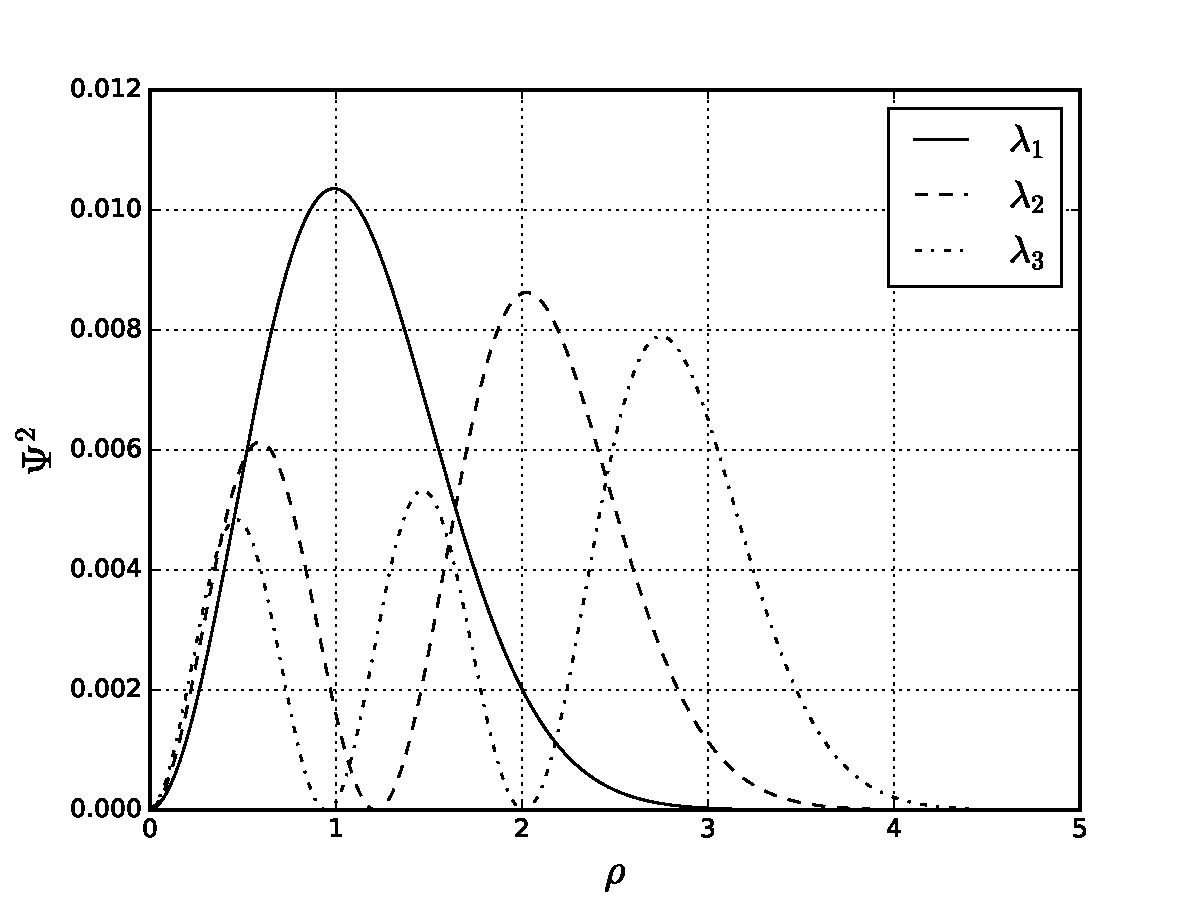
\includegraphics[scale=0.7]{one_electron}
    \caption{One electron}
    \label{fig:one_electron}
  \end{center}
\end{figure}

\begin{figure}
  \begin{center}
    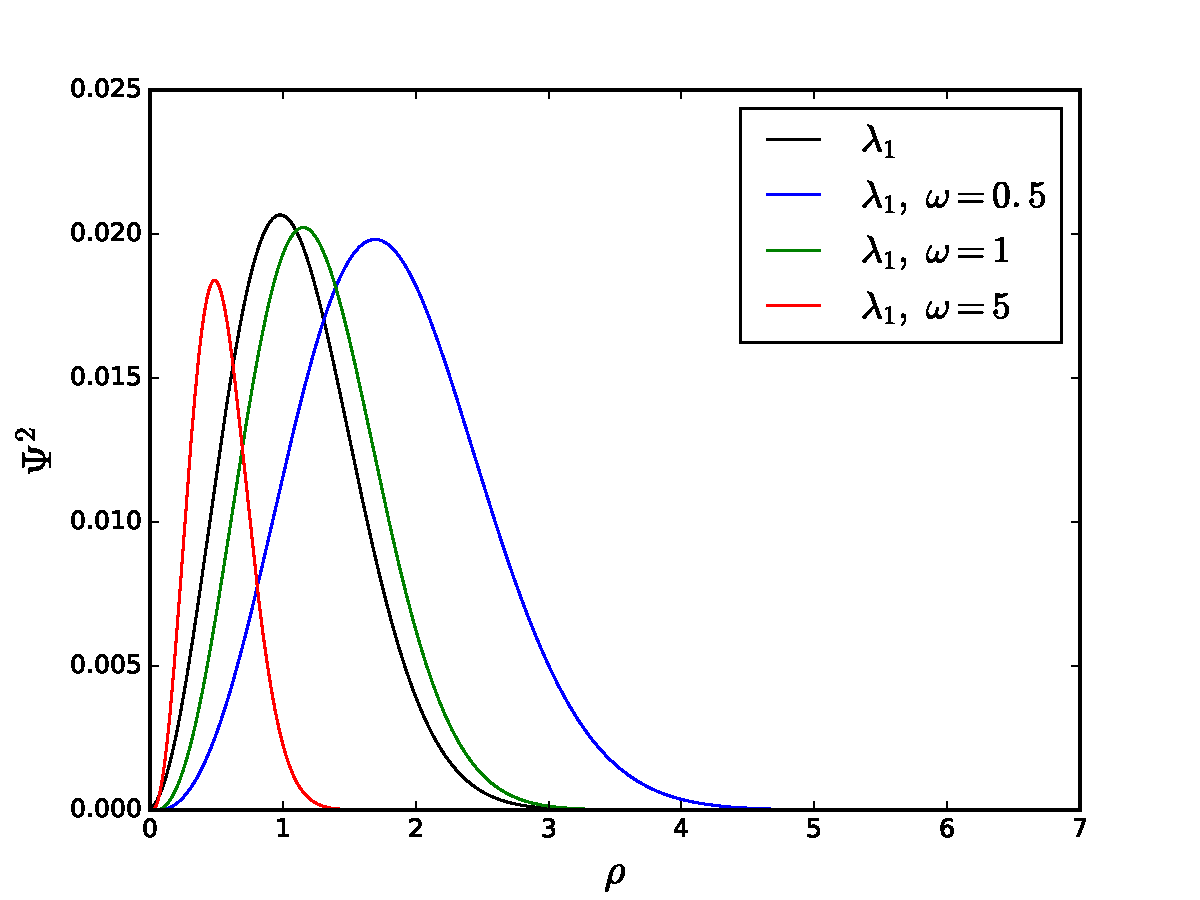
\includegraphics[scale=0.7]{compare}
    \caption{compare}
    \label{fig:compare}
  \end{center}
\end{figure}
\newpage
\begin{figure}
  \begin{center}
    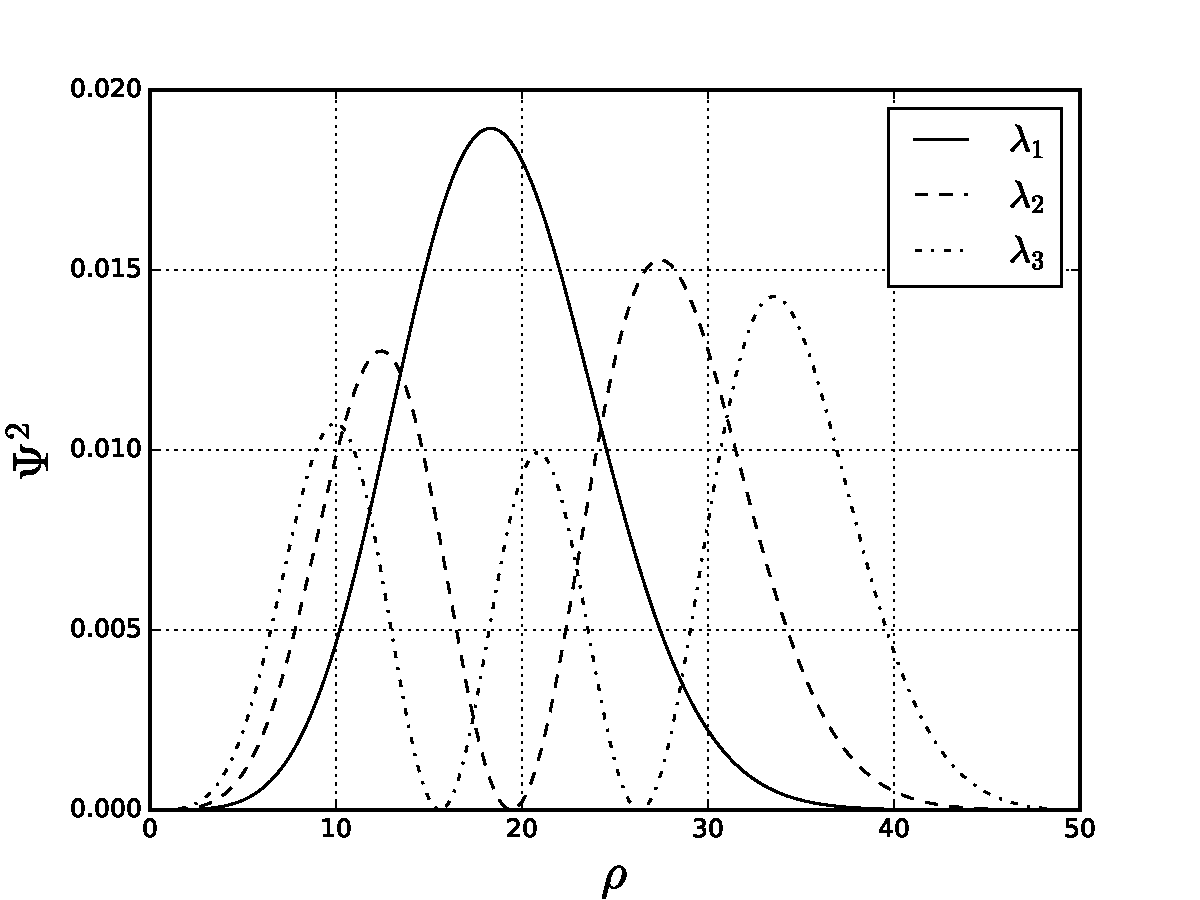
\includegraphics[scale=0.7]{two_001}
    \caption{0.01}
    \label{fig:omega_0.01}
  \end{center}
\end{figure}
\newpage

\begin{figure}
  \begin{center}
    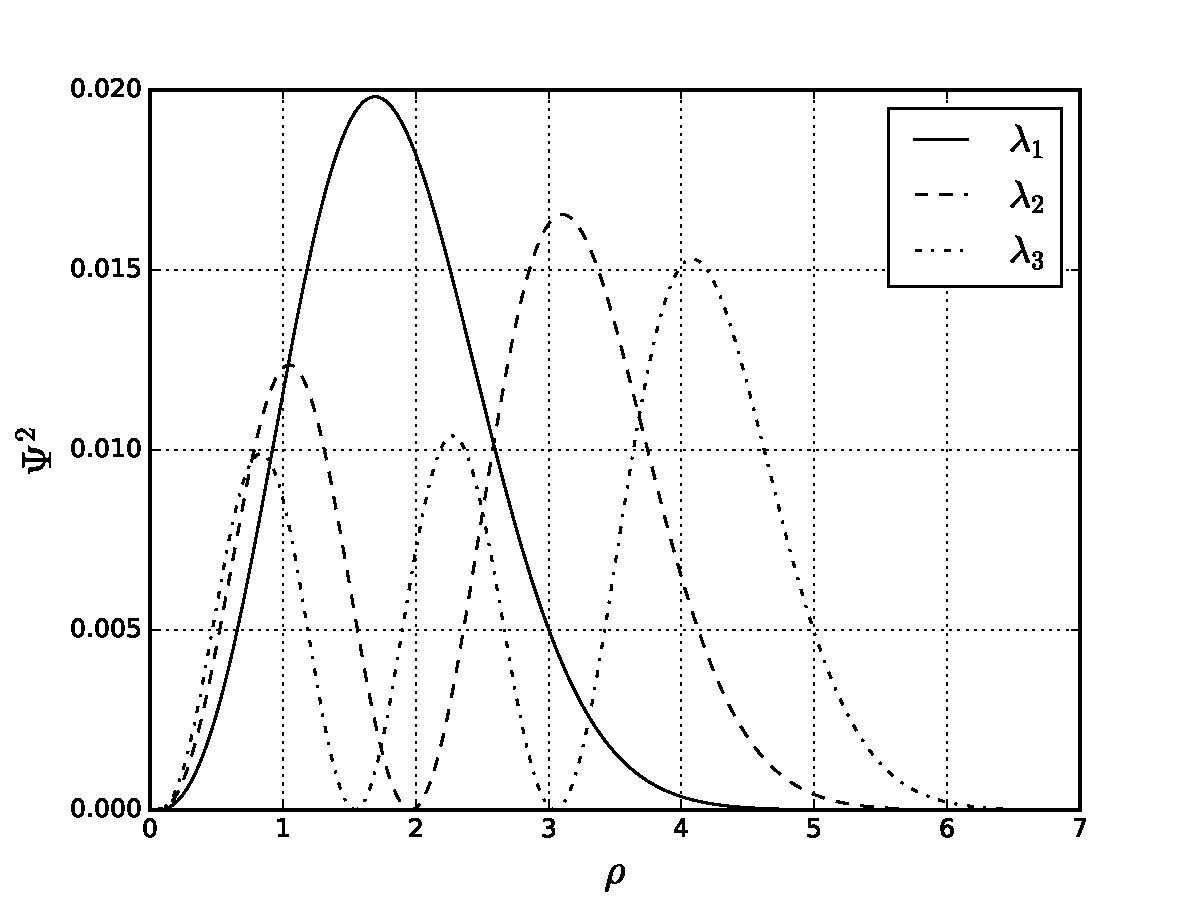
\includegraphics[scale=0.7]{two_05}
    \caption{0.5}
    \label{fig:omega_0.5}
  \end{center}
\end{figure}
\newpage

\begin{figure}
  \begin{center}
    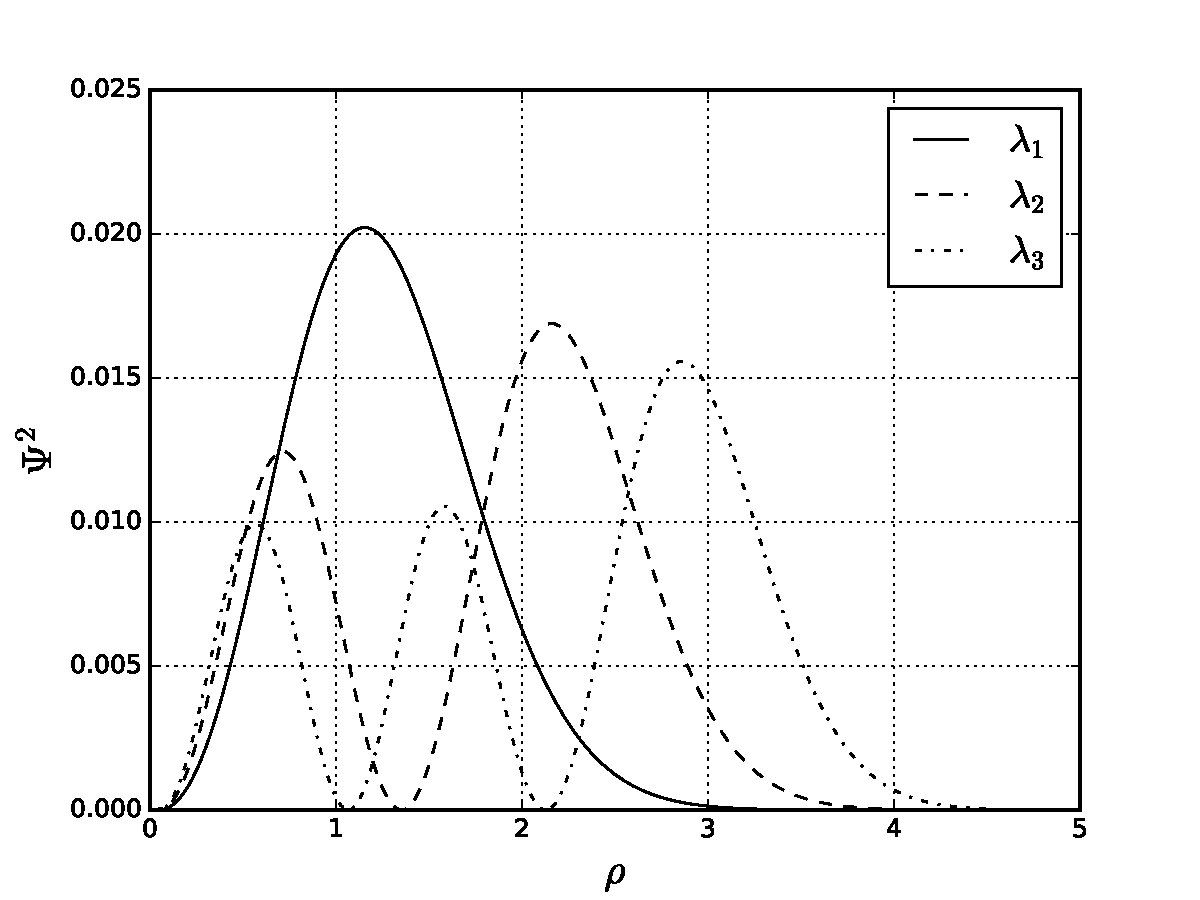
\includegraphics[scale=0.7]{two_1}
    \caption{1}
    \label{fig:omega_1}
  \end{center}
\end{figure}
\newpage

\begin{figure}
  \begin{center}
    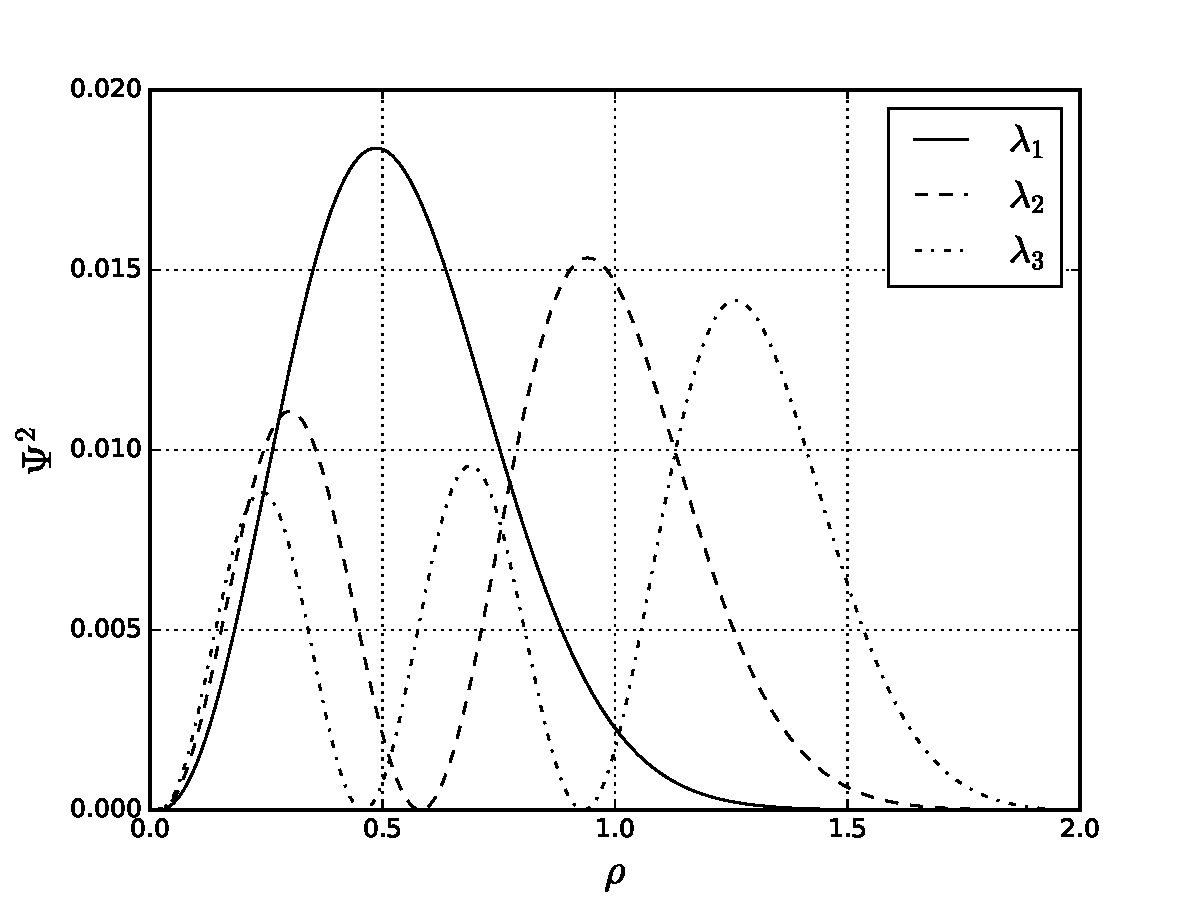
\includegraphics[scale=0.7]{two_5}
    \caption{5}
    \label{fig:omega_5}
  \end{center}
\end{figure}
\newpage


\section{Conclusion and further research}

\newpage
\begin{thebibliography}{2}
\bibitem{one} 
Morten Hjorth-Jensen. 
\textit{Computational Physics
}. 
Lecture Notes Fall 2015, August 2015.
 W. Press, B. Flannery, S. Teukolsky, W. Vetterling, Numerical Recipes in C++, The art of scientific Computing (Cambridge University Press, 1999)

\bibitem{two} 
W. Press, B. Flannery, S. Teukolsky, W. Vetterling 
\textit{Numerical Recipes in C++, The art of scientific Computing}. 
Cambridge University Press, 1999.
 
\end{thebibliography}

\end{document}
